Las siguientes secciones presentan el panorama actual sobre el despliegue y manejo de paquetes de \emph{software}, los problemas de los modelos existentes y la forma en que Nix resuelve algunos de ellos. Posteriormente se discuten los problemas de usabilidad en Nix y los intentos previos por resolverlos; nos enfocamos en su lenguaje \emph{Nixlang}, explicando su naturaleza y cómo se diferencia de otros lenguajes. Se concluye con un resumen de la literatura sobre estudios de usabilidad en lenguajes de programación.

\section{Despliegue de \emph{software}}

La mayoría de los programas se desarrollan pensando en que serán ejecutados en sistemas distintos al que los vio nacer. El conjunto de actividades orientadas a llevar un artefacto de \emph{software} desde el entorno de desarrollo hasta las computadoras del usuario final, y a garantizar su correcto funcionamiento a lo largo de todo su ciclo de vida ---instalación, actualización, configuración y eventual desinstalación---, constituye el campo de interés del despliegue de \emph{software}~\cite{mantylaSoftwareDeploymentActivities2011,Dolstra2006}. Contrario a la percepción común de que desplegar un programa se reduce a ``copiar archivos'', Mäntylä y Vanhanen~\cite{mantylaSoftwareDeploymentActivities2011} documentan, a partir de un estudio de caso en cuatro empresas, que se trata de un proceso multifacético que involucra la interacción con el cliente, la integración con sistemas externos y la configuración del entorno de ejecución; complejidad que se acentúa cuando el producto depende de un modelo de datos particular o de una integración estrecha con otros sistemas.

Esta noción amplia de despliegue está estrechamente vinculada con el campo del Manejo de Configuración de \emph{Software} (SCM, por sus siglas en inglés), disciplina orientada a preservar la integridad de un producto a lo largo de su evolución mediante la identificación, el control y la auditoría de los cambios realizados sobre sus componentes~\cite{bersoffSoftwareConfigurationManagement1978}. Dolstra~\cite{Dolstra2006} formaliza la relación entre ambos campos al señalar que la ejecución correcta de un artefacto de \emph{software} no depende únicamente de su código fuente, sino del contexto que lo rodea ---\emph{hardware}, sistema operativo, bibliotecas y demás dependencias---; desplegar un programa consiste, entonces, en reconstruir fielmente dicho contexto en cada entorno de destino.

Para lidiar con esta dependencia del contexto han surgido distintas familias de herramientas, cada una centrada en una faceta particular del problema: los manejadores de paquetes, que automatizan la instalación y resolución de dependencias dentro de un entorno compartido; las herramientas de virtualización y contenedores, que empaquetan la aplicación junto con su entorno de ejecución para aislarla del resto del sistema~\cite{Sobieraj2024,Lingayat2018}; los sistemas de construcción (\emph{build systems}), que transforman el código fuente en artefactos ejecutables de forma reproducible; y las herramientas de gestión de configuración, orientadas al aprovisionamiento y mantenimiento de servidores completos~\cite{Zwinger2026}. Estas categorías no son mutuamente excluyentes, sino que solo interactúan en diferentes fases con las mismas unidades de contenido: el paquete de \emph{software}.

\section{Paquetes de \emph{software}}

``Uno de los principios fundamentales de la ingeniería de \emph{software} es promover la reutilización sobre la reimplementación de soluciones existentes.''~\cite{jaimeAnalysisEvolutionDependencies} Pueden encontrarse indicios de esta práctica desde los primeros programas aritméticos de 1947~\cite{goldstainPlanningCodingProblems1947}, y hoy en día ha evolucionado hasta el punto en que buena parte de las herramientas usadas por desarrolladores de \emph{software} dependen, en mayor o menor medida, de piezas de código desarrolladas por terceros, como React, Vue.js o Scikit-learn~\cite{jaimeAnalysisEvolutionDependencies}.

A este conjunto de código fuente, binarios y otros archivos reutilizables se le conoce como librerías, dependencias o paquetes~\cite{mensSoftwareEcosystemsTooling2023}, y constituyen un método eficaz para reducir el tiempo de desarrollo y permitir a los desarrolladores enfocarse en el producto final. Además, se percibe que el código de los paquetes es de mejor calidad, probablemente porque gran parte de ellos es de código abierto, es decir, revisado y modificado por múltiples desarrolladores~\cite{societyGuideSoftwareEngineering2026}.

El uso de código de terceros se ha convertido en una práctica extendida: en 2026, la compañía Black Duck~\cite{blackduck2026OSSRAReport} ---que ofrece herramientas para evaluar la seguridad de paquetes de código abierto en proyectos de \emph{software}--- realiza un estudio sobre 2,843 proyectos de distintas industrias, en el que encuentra que el 98\% de ellos utiliza paquetes de código abierto, con un promedio de 1,180 paquetes por proyecto; ambas cifras superiores a las reportadas en un estudio previo de 2025. Este crecimiento no se limita al uso de bibliotecas, sino también a su cantidad dentro de cada proyecto: un ejemplo es el navegador Mozilla Firefox, cuyo árbol de dependencias supera los 20,000 paquetes (Anexo~\ref{Appendix5}), complejidad que se ilustra en la Figura~\ref{figure3}, donde cada punto representa un paquete coloreado por ecosistema: \texttt{npm} en azul, \texttt{cargo} en naranja, \texttt{pypi} en verde y otros en gris; el punto negro central es el propio repositorio de Firefox. A simple vista se puede intuir que mantenerlos manualmente no resultaría divertido para ningún desarrollador.

\begin{figure}[htbp]
\centering
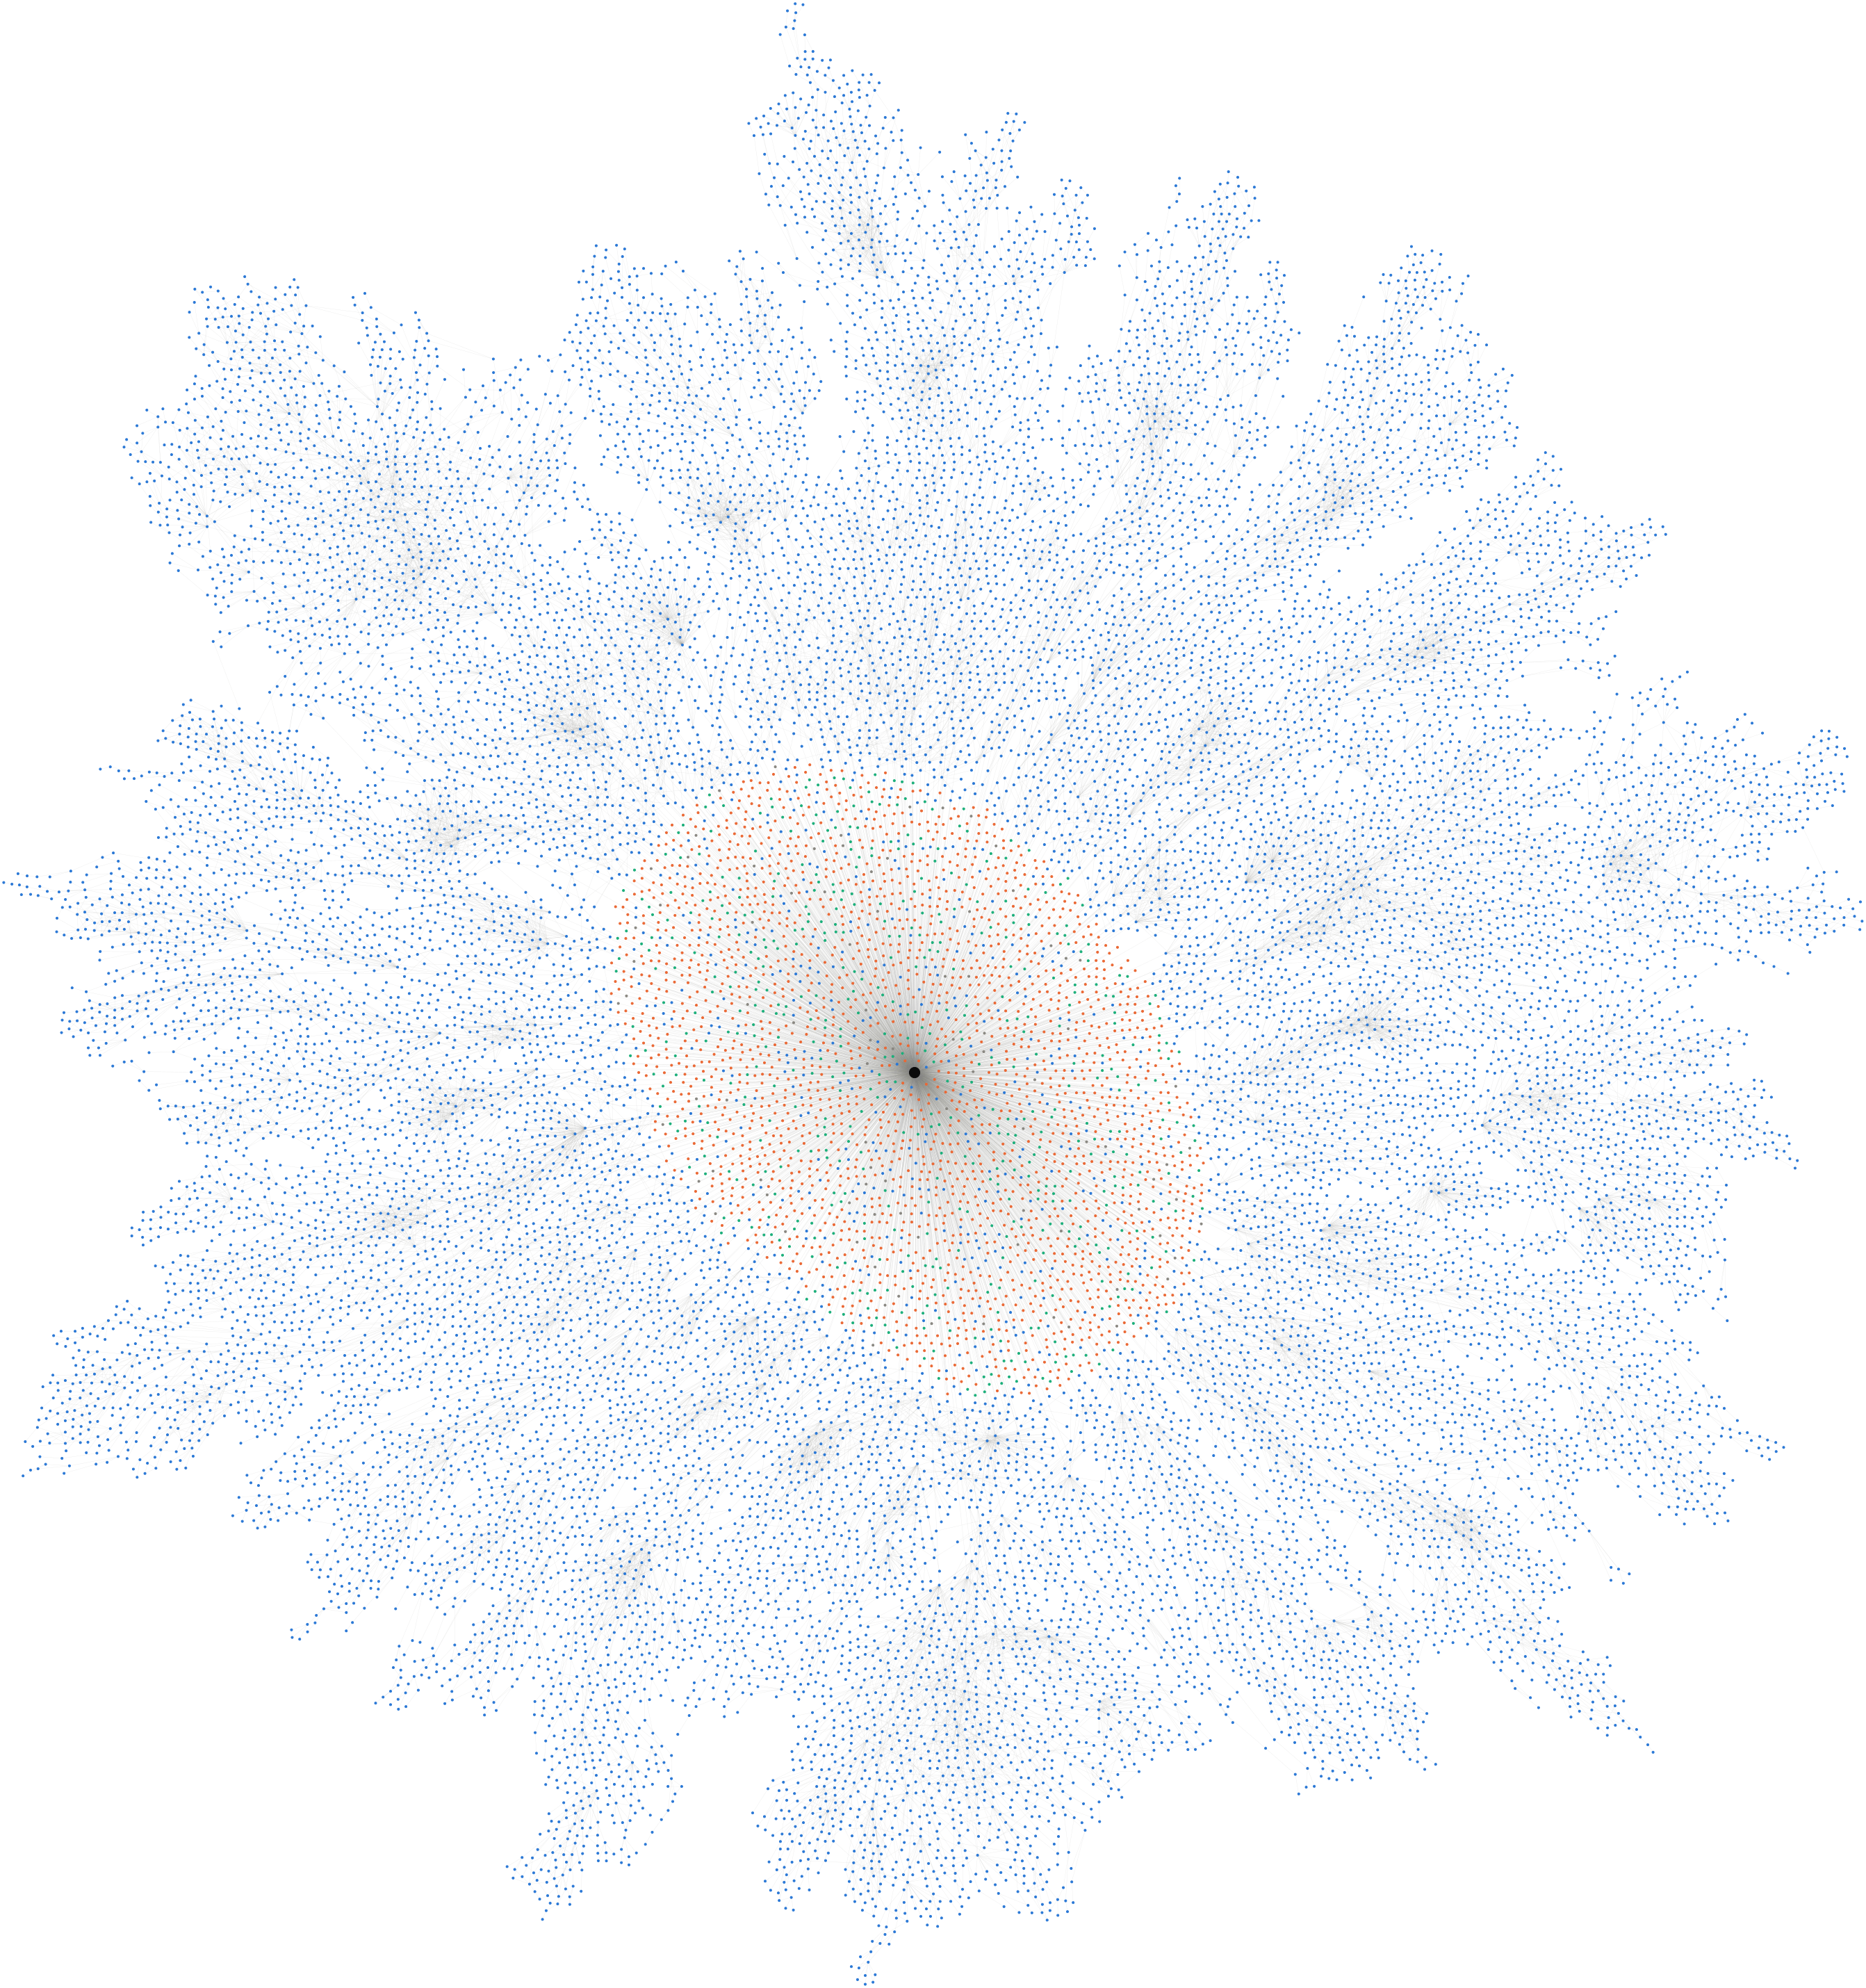
\includegraphics[width=0.85\textwidth]{Figure3.png}
\caption{Grafo completo de dependencias de Firefox (21,295 paquetes, 37,926 relaciones \texttt{DEPENDS\textunderscore{}ON}).}
\label{figure3}
\end{figure}

La Figura~\ref{figure3} revela una característica esencial de los paquetes, y es que estos, a su vez, pueden depender de otros paquetes; formando un \emph{grafo de dependencias de software}, donde paquetes son conectados por vértices dirigidos que simbolizan relaciones ``depende de''~\cite{kikasStructureEvolutionPackage2017}. Es esta estructura de datos la que muchos manejadores de paquetes utilizan para saber qué instalar y en qué orden~\cite{Gibb2026}, como se discute en la Sección~\ref{manejadores_de_paquetes}. Esta misma estructura, además, permite clasificar los diferentes tipos de paquetes.

\subsection{Clasificación de paquetes}

Los paquetes se pueden clasificar según su relación con el paquete principal (la aplicación que el usuario desea usar)~\cite{Gibb2026}:

\begin{itemize}
\item \textbf{Directas}: Paquetes que el paquete principal declara explícitamente que necesita.
\item \textbf{Indirectas}: Paquetes que son, a su vez, dependencias de las dependencias directas, sin ser requeridos por el paquete principal.
\item \textbf{Opcionales}: Paquetes que el autor sugiere tener instalados, pero cuya ausencia no compromete la funcionalidad principal de la aplicación.
\end{itemize}

En la Figura~\ref{figure4} se puede observar un grafo de dependencias que ejemplifica las tres categorías; cada punto representa un paquete: dependencias directas en amarillo, indirectas en azul y opcionales en rojo.

\begin{figure}[htbp]
\centering
\includegraphics[width=0.6\textwidth]{Figure4}
\caption{Grafo de dependencias de \texttt{tu aplicación}.}
\label{figure4}
\end{figure}

Una segunda clasificación de los paquetes atiende a la forma en que son referenciados por la aplicación objetivo~\cite{Dolstra2006}. Esta distinción surge de la naturaleza misma de la ejecución de programas: para que un programa se ejecute, su código fuente debe traducirse a instrucciones binarias que el procesador pueda interpretar, proceso que incluye una fase de enlazado o \emph{linking}, en la cual se resuelven las referencias que el programa hace a funciones y variables definidas en otros paquetes~\cite{beazleyStorySharedLibraries2001}. Esta fase es especialmente visible en lenguajes como \texttt{C}, aunque el \emph{linking} también está presente en otros lenguajes compilados e interpretados; en estos últimos, sin embargo, la resolución ocurre en tiempo de ejecución, a cargo del intérprete, en lugar de quedar fijada de antemano en el ejecutable. Según el momento en que ocurre esta resolución, los paquetes que actúan como bibliotecas se clasifican en estáticos o dinámicos.

\subsubsection{Librerías estáticas}

La opción más sencilla para que un ejecutable tenga acceso a las funcionalidades de una librería es copiar el contenido de la librería en el código fuente. A las librerías que son referenciadas de esta forma se les conoce como \textbf{estáticas}, debido a que una vez referenciadas, su código no cambia a menos que se compile nuevamente~\cite{roucariesStaticLinkingPitfalls2025}.

En el caso de \texttt{C}, el proceso se hace evidente al traducir cada archivo fuente en un archivo objeto (\emph{object file} \texttt{.o}); estos artefactos cuentan dentro de sí con una tabla de símbolos de librerías externas pendiente por resolver. Es necesario resolver estos símbolos para producir el ejecutable, y es en este punto donde se copian los contenidos de las librerías estáticas~\cite{beazleyStorySharedLibraries2001}.

El \emph{linker} toma el ejecutable en construcción, identifica los símbolos que aún no están definidos y copia dentro del binario final únicamente las definiciones que son mencionadas en el código fuente~\cite{usenixassociation1986SummerUSENIX1986}. El resultado es un ejecutable autocontenido, que no depende de que la biblioteca esté presente en la computadora donde se ejecuta~\cite{beazleyStorySharedLibraries2001}.

Esta característica trae ventajas y desventajas. Viendo lo positivo, \textbf{produce binarios portables y con un comportamiento predecible}, ya que no existe la posibilidad de que se utilice código diferente al probado por el desarrollador y evita la sobrecarga de resolver símbolos cada vez que el programa se ejecuta~\cite{beazleyStorySharedLibraries2001}. Esta característica los hace sencillos de distribuir, porque su instalación se limita a copiar los ejecutables en la computadora destino\footnote{En realidad el proceso puede involucrar otras actividades como la configuración de variables de entorno y creación de archivos de configuración, pero pueden considerarse triviales comparado a la resolución de dependencias~\cite{Dolstra2006}}.

Por otro lado, cada ejecutable que usa la misma biblioteca contiene su propia copia del código, lo que incrementa el tamaño en disco y el consumo de memoria cuando varios programas la usan simultáneamente~\cite{usenixassociation1986SummerUSENIX1986}; también obliga a recompilar y redistribuir cada ejecutable ante cualquier actualización o corrección de la biblioteca, incluidos parches de seguridad~\cite{beazleyStorySharedLibraries2001}.

\subsubsection{Librerías dinámicas}

Como respuesta a los pesados binarios del enlazado estático, ¿qué tal si en vez de copiar el código solo indicamos en qué archivo encontrarlo? Así muchos ejecutables podrían ``compartir'' las funcionalidades de la librería sin duplicarla. Hemos descubierto el \textbf{enlazado dinámico}~\cite{usenixassociation1986SummerUSENIX1986}.

Las \textbf{bibliotecas dinámicas} (o compartidas, \emph{shared libraries}; \texttt{.so} en Unix, \texttt{.dll} en Windows, \texttt{.dylib} en macOS) posponen la resolución de símbolos hasta la ejecución o, incluso, hasta la primera vez que la función es invocada (\emph{lazy binding})~\cite{beazleyStorySharedLibraries2001}. En lugar de copiar el código de la biblioteca dentro de cada ejecutable, el binario final solo almacena una referencia a ella; es el cargador dinámico del sistema operativo (\emph{dynamic loader}) quien, al iniciar el programa, localiza la biblioteca en el sistema, la mapea en el espacio de memoria del proceso y completa las referencias pendientes mediante tablas de relocalización y código independiente de posición (\emph{Position Independent Code}, PIC)~\cite{beazleyStorySharedLibraries2001}.

Esta solución ofrece ciertos beneficios: el sistema operativo puede mantener una única copia de la biblioteca en memoria física y compartirla entre todos los procesos que la usan, reduciendo el consumo de RAM y el tamaño de los ejecutables en disco; además, una biblioteca puede corregirse o actualizarse sin necesidad de recompilar las aplicaciones que la consumen, siempre que se preserve su interfaz~\cite{roucariesStaticLinkingPitfalls2025}.

Esta misma flexibilidad introduce el problema opuesto al de las bibliotecas estáticas: la aplicación depende de que, en la computadora donde se ejecute, exista una versión de la biblioteca compatible con la que se usó al compilarla, situación que puede derivar en conflictos cuando distintas aplicaciones del mismo sistema requieren versiones incompatibles entre sí~\cite{roucariesStaticLinkingPitfalls2025}, como se ilustró previamente en la Figura~\ref{figura1}.

Las clasificaciones desarrolladas no son las únicas: distintos ecosistemas introducen conceptos adicionales, como los paquetes \emph{peer} que introduce \texttt{npm}~\cite{Gibb2026}.

\section{Manejadores de paquetes al rescate}\label{manejadores_de_paquetes}

De las secciones anteriores debe quedar claro que instalar una aplicación junto con sus dependencias no es un problema trivial. Ante el auge en la disponibilidad y uso de paquetes descrito previamente, también ha surgido una plétora de herramientas orientadas a administrar la creciente complejidad derivada del tamaño de los proyectos.

\subsection{Evolución y taxonomía de los modelos existentes}

A partir de mediados de la década de los 2000, se produjo lo que se ha descrito como una ``explosión cámbrica'' de soluciones, donde prácticamente cada sistema operativo y lenguaje de programación desarrolló su propio manejador de paquetes~\cite{Gibb2026}; con el tiempo se fueron diferenciando bajo tres ejes principales:

\begin{enumerate}
\item \textbf{Por el tipo de artefacto}

\begin{itemize}
\item \textbf{Manejadores binarios:} Descargan binarios precompilados de servidores centrales y los ubican en rutas específicas del sistema. Su ventaja es la velocidad, pero dependen de que el binario haya sido construido para una arquitectura y versión de sistema operativo exacta~\cite{Zwinger2026}; ejemplos incluyen \texttt{APT}, \texttt{RPM} y \texttt{Pacman}.
\item \textbf{Manejadores basados en fuentes:} Copian el código fuente y producen los binarios localmente~\cite{Zwinger2026}. Esto permite una personalización extrema y optimización para el \emph{hardware}, pero a costa de tiempos de despliegue significativamente mayores~\cite{Dolstra2006}; ejemplos incluyen \texttt{BSD Ports} o \texttt{Portage}.
\end{itemize}
\item \textbf{Por el alcance del ecosistema}

\begin{itemize}
\item \textbf{Manejadores de sistema:} Administran el sistema operativo completo (p. ej., DNF para Red Hat, APT para Debian). Tienden a ser más conservadores, priorizando un conjunto de paquetes coordinado y coherente, lo que a menudo causa que las versiones de las librerías se retrasen respecto a las últimas novedades~\cite{Gibb2026}.
\item \textbf{Manejadores de lenguaje:} Distribuyen librerías para desarrolladores de lenguajes específicos (p. ej., pip para Python, Cargo para Rust, npm para JavaScript). Priorizan la frescura de las versiones, pero suelen ignorar las dependencias externas del sistema (como drivers o librerías de C), asumiendo que estas ya están presentes~\cite{Gibb2026}.
\end{itemize}
\item \textbf{Por la resolución de dependencias:} Dependiendo del tipo de algoritmo utilizado para resolver las dependencias necesarias, a menudo utilizando algoritmos \emph{SAT solvers} para encontrar las versiones compatibles, un proceso que es inherentemente NP-completo. Manejadores como Nix evaden este problema permitiendo solo una versión válida~\cite{Dolstra2006}.
\end{enumerate}

\subsection{El problema de fondo: el paradigma imperativo}

A pesar de su utilidad, los modelos tradicionales comparten un defecto estructural: operan bajo un \textbf{paradigma de despliegue imperativo}. En este modelo, las acciones de instalación o actualización se realizan ``en el lugar'' (\emph{in-place}), modificando destructivamente el estado del sistema operativo~\cite{Courts2013}. Esta mutación del entorno global conlleva problemas críticos que limitan la fiabilidad del \emph{software}:

\begin{itemize}
\item \textbf{Conflictos de dependencias (``Dependency Hell''):} Al intentar satisfacer a múltiples aplicaciones en un entorno global único, surge el problema del ``diamante de dependencias''. Si la aplicación A requiere la versión 1.0 de una librería y la aplicación B requiere la 2.0, el sistema se ve forzado a elegir una sola, rompiendo potencialmente la otra aplicación~\cite{Zwinger2026}.
\item \textbf{Falta de reproducibilidad:} Debido a que el proceso de construcción suele tener acceso a todo el \emph{software} instalado en la máquina (entradas no declaradas), es común que un paquete se compile correctamente en una computadora pero falle en otra debido a sutiles diferencias en el entorno~\cite{Courts2013}.
\item \textbf{Actualizaciones destructivas y falta de reversión:} Dado que las actualizaciones sobrescriben archivos existentes, si un proceso falla a mitad de camino o la nueva versión es inestable, el sistema puede quedar en un estado inconsistente. No suele haber una forma sencilla de realizar un \textbf{rollback} atómico al estado anterior~\cite{Dolstra2006}.
\item \textbf{Fragmentación de herramientas:} Los proyectos multilingües modernos se ven obligados a coordinar múltiples manejadores de paquetes \emph{ad-hoc} (p. ej., usar Cargo, pip y APT simultáneamente), lo que oculta vulnerabilidades de seguridad y dificulta el despliegue portátil~\cite{Gibb2026}.
\end{itemize}

\section{La virtualización es la solución\dots{} o no}

En paralelo al nacimiento y evolución de los manejadores de paquetes, en otra rama crecía una alternativa: la virtualización. Esta nació para compartir los recursos de \emph{hardware} de una misma máquina entre varios usuarios~\cite{kozirisFiftyYearsEvolution2015}, pero con la llegada de la nube demostró ser un medio ideal para desplegar \emph{software} de forma reproducible~\cite{Sobieraj2024}.

Docker fue la herramienta que popularizó la virtualización como forma de empaquetar (o ``contenerizar'') aplicaciones. Su idea es sencilla: en vez de simular una computadora entera, los contenedores se ejecutan directamente sobre el sistema anfitrión, y es el propio kernel el que le da a cada proceso la ilusión de estar solo en su propia computadora. Para ello se apoya en dos mecanismos de Linux: los \emph{namespaces}, que restringen lo que un proceso puede ver (procesos, sistema de archivos, red y usuarios), y los \emph{cgroups}, que restringen cuánto puede usar (CPU, memoria, disco)~\cite{Sobieraj2024}. Por eso un contenedor arranca mucho más rápido que una máquina virtual~\cite{Lingayat2018}.

Esta virtualización ligera dio paso a un nuevo modelo de empaquetado: distribuir la aplicación junto con el ambiente completo en el que debe ejecutarse, llamándolos ``contenedores''. Para no duplicar ese ambiente, Docker introduce el concepto de ``imágenes'' como sistemas de archivos por capas, donde cada capa representa un cambio en el sistema de archivos de tal manera que si dos contenedores realizan los mismos cambios, esa capa se puede compartir entre varios contenedores~\cite{UnderstandingImageLayers}.

Una capa solo se reutiliza si es idéntica, y como cada una se construye sobre las anteriores, modificar una instrucción invalida esa capa y todas las siguientes. Así, dos imágenes que instalan la misma librería sobre bases distintas terminan guardando copias separadas de los mismos archivos, lo que en la práctica llena los registros de imágenes de datos duplicados~\cite{zhaoEndtoendHighperformanceDeduplication2024a}. De igual forma, aunque los contenedores son más ligeros que una máquina virtual, siguen teniendo un costo de rendimiento frente a la ejecución nativa~\cite{Giallorenzo2021}, que se agrava en Windows y macOS, donde Docker necesita una máquina virtual de Linux para funcionar~\cite{Sobieraj2024}.

\section{Nix como solución}

La disyuntiva tradicional obligaba a elegir entre manejadores que arriesgan conflictos en el entorno global o soluciones de virtualización (contenedores) que evitan conflictos duplicando entornos completos a costa de almacenamiento y memoria, como se ve en la Figura~\ref{figura1} con \texttt{Programa 1} y \texttt{Programa 2} dependiendo de \texttt{FOO}.

\begin{figure}[htbp]
\centering
\includegraphics[width=0.9\textwidth]{Figure5}
\caption{Peores casos de resolución de dependencias en a) los modelos de manejadores de paquetes y b) virtualización.}
\label{figura5}
\end{figure}

En este contexto surge \textbf{Nix}, que propone una tercera vía: un \textbf{modelo de despliegue puramente funcional}; construir un paquete debería ser como una función pura: dadas las mismas entradas debería devolver siempre las mismas salidas. Lo logra al fusionar la eficiencia de los manejadores de paquetes con el aislamiento de la virtualización~\cite{Dolstra2006}.

\subsection{Cómo lo soluciona}

Nix resuelve ambos problemas de manejadores de paquetes y virtualización a la vez mediante el mismo mecanismo: \textbf{los hashes}. Si cada paquete recibiera un nombre único, tener dos versiones de una librería sería posible porque a ojos de la computadora son 2 programas diferentes; también se eliminaría el problema de la duplicación, porque los identificadores únicos permiten saber si 2 paquetes dependen de la misma exacta dependencia, y compartirla. Esos nombres únicos son hashes que Nix agrega como prefijos a todo recurso, así que el ejecutable, en vez de llamarse \texttt{firefox}, se llamaría \texttt{wkgaavd2hzy9kmw0z30a8yxw796nfhx5-\allowbreak{}firefox}~\cite{Dolstra2006}.

Sin embargo, los hashes solo son fiables si el sistema asegura que sean reproducibles, es decir, dados siempre el mismo paquete e instrucciones, se le asigne el mismo hash, sin importar la computadora donde es ejecutado. Es ahí donde para Nix cobra sentido adoptar un modelo funcional, porque busca resolver un problema muy parecido con las funciones puras. El resto de esta sección detalla los mecanismos que hacen esto posible, así como el lenguaje mediante el cual se describen.

\subsection{Implementación}

Para permitir resolver las falencias de los manejadores de paquetes y la virtualización, el modelo de Nix, propuesto por Dolstra~\cite{Dolstra2006}, introduce sus propios componentes que son resumidos en la Figura~\ref{figura6}: todo empieza con un archivo en \textbf{Nixlang}; al ser evaluado, se produce un archivo de \textbf{derivación} \texttt{.drv} con las instrucciones exactas de cómo construir lo que solicita el usuario para un sistema específico.

La derivación es guardada en un espacio común conocido como la \textbf{Nix Store}. Nix solo interactúa con cosas presentes en la Nix Store para reducir efectos inesperados, así que si no cuenta con un recurso, primero lo descarga y coloca aquí. Es en este proceso donde al recurso se le asigna el \textbf{hash} mencionado anteriormente.

Una vez se cuenta con los recursos necesarios, Nix construye el paquete en ambientes aislados por medio de una virtualización ligera para asegurar la reproducibilidad. Todo lo anterior mencionado es orquestado por el \textbf{Nix Daemon}.

\begin{figure}[htbp]
\centering
\includegraphics[width=\textwidth]{Figure6}
\caption{Diagrama simplificado de los componentes principales de Nix.}
\label{figura6}
\end{figure}

Como se puede ver, todos los mecanismos de Nix están orientados a una misma meta: maximizar la reproducibilidad, porque al seguir los mismos pasos bajo el mismo ambiente y condiciones, debe llevar al mismo resultado. Las secciones de abajo buscan explicar un poco mejor cómo cada parte lo logra.

\subsubsection{Derivaciones}

Para construir un paquete, es necesaria una receta detallada de cómo construirlo. A esas recetas Nix les llama \textbf{derivaciones}. En concreto, una derivación es un archivo \texttt{.drv} con una especificación detallada para construir un paquete en un sistema específico (arquitectura y sistema operativo); especificando mediante qué programa se debe construir (\emph{builder}), con qué argumentos y variables de entorno y de qué otras derivaciones depende. Así es, las dependencias son representadas por derivaciones, no paquetes; de esta manera, si no se cuenta con el paquete pero sí con la derivación, se puede construir localmente~\cite{Dolstra2006}.

Estas recetas se pueden ver como funciones puras (Figura~\ref{figura7}): \textbf{los parámetros} son todas las cosas que nuestro paquete necesita para construirse y correrse, \textbf{el cuerpo} contiene las instrucciones en \texttt{bash} para construir el paquete, y la \textbf{salida} es el paquete junto con el hash único que lo identifica y del que discutimos a continuación cómo se computa.

\begin{figure}[htbp]
\centering
\includegraphics[width=0.7\textwidth]{Figure7}
\caption{Comparación visual de las derivaciones con las funciones puras.}
\label{figura7}
\end{figure}

\subsubsection{Hashes}

Considerando que el modelo de Nix trabaja alrededor de derivaciones, y que cada derivación es como una función pura, produciendo la misma salida dados los mismos parámetros, computar un identificador único para cada paquete es relativamente sencillo: basta con hacer un hash criptográfico de la combinación de todos los parámetros utilizados: código fuente, dependencias, banderas de compilación y el propio script de construcción~\cite{Dolstra2006}. Como el hash depende exclusivamente de esos insumos, dos construcciones con los mismos insumos producen exactamente el mismo hash y, por tanto, el mismo paquete, sin importar en qué máquina se ejecuten; esta propiedad es la que permite sustituir binarios ya construidos entre computadoras distintas, y ha sido validada empíricamente reconstruyendo más de 700 mil paquetes de Nixpkgs con tasas de reproducibilidad binaria de entre 69\% y 91\%~\cite{Malka2025}.

Modificar cualquier insumo ---incluida una dependencia transitiva--- cambia el hash resultante y con él el paquete, de modo que la noción de versionado semántico no existe realmente en Nix, pudiendo existir varios \texttt{node-22} por usar parámetros ligeramente diferentes.

\subsubsection{Ambientes aislados}

Nix ejecuta cada construcción dentro de un ambiente aislado que restringe el sistema de archivos visible a únicamente las rutas del store declaradas como insumos, y deshabilita el acceso a la red salvo que la derivación lo declare explícitamente~\cite{Dolstra2006}. Esta forma de virtualización, más ligera que la de una máquina o un contenedor completo, impide que dependencias no declaradas del sistema anfitrión ---una biblioteca instalada globalmente, una variable de entorno, un archivo de configuración--- se filtren silenciosamente en el resultado de la construcción, condición necesaria para que el hash calculado sea reproducible en cualquier otra máquina~\cite{Dolstra2006,Malka2025}.

\subsubsection{Nix Store}

Incluso si todos los componentes anteriores producen paquetes reproducibles, nada evita que un usuario o proceso los sobreescriba sin actualizar el hash, llevando a un estado ilegal donde el hash ya no es el identificador de los contenidos a los que acompaña. Para evitar manipulación externa, cualquier recurso con el que Nix interactúa es copiado en un directorio de solo lectura llamado la \textbf{Nix Store}. Cualquier contenido dentro de la Nix Store es inmutable y cualquier inserción o eliminación se hace por medio de solicitudes al \textbf{Nix Daemon}~\cite{Dolstra2006}.

Es aquí donde el hash descrito antes es usado, al ser el prefijo del nombre de cualquier archivo y carpeta dentro de la store, identificando de forma inequívoca su contenido (Figura~\ref{figura6}), lo que permite que Nix trate al sistema operativo completo, en el caso de NixOS, como una colección de artefactos versionados dentro de esta misma estructura~\cite{Dolstra2008}.

\subsubsection{Nixlang}

Nixlang es, en última instancia, un medio declarativo para describir y componer derivaciones: cualquier expresión Nix se evalúa hasta producir una o más derivaciones, que Nix evalúa para obtener las rutas de salida correspondientes en el store~\cite{Dolstra2006}. Es un lenguaje de dominio específico funcional y de evaluación perezosa, con tipado dinámico y una sintaxis descrita en ocasiones como JSON con funciones~\cite{NixdevDocumentation}. Estos dos últimos rasgos ---el paradigma funcional y la evaluación perezosa--- emergen como respuesta al diseño funcional de las derivaciones.

En la actualidad se ha popularizado el uso de los Flakes~\cite{2025CommunitySurvey}, un formato estructurado para escribir con Nixlang que ofrece ventajas al agregar más salvaguardas para preservar el determinismo~\cite{NixdevDocumentation}.

Antes de examinar cómo estas propiedades inciden en la usabilidad de Nixlang, conviene precisar qué significan en términos de teoría de lenguajes de programación.

\section{Fundamentos de lenguajes de programación}

Esta sección introduce tres nociones de diseño de lenguajes ---el contraste entre paradigma imperativo y funcional, la evaluación perezosa y la noción de lenguaje de dominio específico--- que sirven de base conceptual para analizar tanto Nixlang como el eDSL propuesto en este trabajo.

\subsection{Imperativo vs. funcional}

En un lenguaje imperativo, un programa es una secuencia de instrucciones que modifican explícitamente el estado de la máquina ---variables, registros, archivos--- mediante asignaciones y efectos secundarios; es el modelo que siguen la mayoría de los lenguajes de propósito general (\texttt{C}, Python, JavaScript) y el que, según Dolstra~\cite{Dolstra2008}, comparten los manejadores de paquetes y las herramientas de gestión de configuración tradicionales, cuyas actualizaciones sobrescriben destructivamente el estado del sistema. En un lenguaje funcional, en cambio, un programa se construye componiendo funciones matemáticas puras sobre valores inmutables: dada la misma entrada, una función siempre produce la misma salida, sin alterar ningún estado externo, propiedad conocida como transparencia referencial~\cite{Hudak1989}. Es precisamente esta noción, trasladada del diseño de lenguajes al despliegue de \emph{software}, la que origina el modelo de Nix descrito en la sección anterior: una derivación se comporta como una función pura; es por ello que el lenguaje para describirlas sigue esa misma disciplina.

\subsection{Laziness}

La evaluación perezosa (\emph{lazy evaluation}) pospone el cómputo de una expresión hasta el momento en que su valor es efectivamente requerido, en contraste con la evaluación estricta (\emph{eager}), que calcula cada expresión tan pronto como es posible~\cite{Hudak1989}. Nixlang hereda esta propiedad de su linaje funcional: un atributo dentro de un archivo de configuración puede referenciar a otro definido más adelante, o incluso a sí mismo de forma indirecta, sin provocar un ciclo infinito, siempre que exista un punto fijo que Nix pueda resolver perezosamente~\cite{Dolstra2006}. Esta característica habilita patrones extendidos en el ecosistema, como los \emph{overlays} que modifican paquetes ya definidos, pero también introduce un modelo mental ---la ausencia de un orden de evaluación explícito--- ajeno a la mayoría de los lenguajes imperativos con los que suelen familiarizarse primero los nuevos usuarios.

\subsection{DSL \& eDSL}

Un \textbf{lenguaje de dominio específico} (DSL, por sus siglas en inglés) es un lenguaje diseñado para un dominio de aplicación particular que, a cambio de renunciar a la generalidad de un lenguaje de propósito general (GPL), ofrece en teoría mayor expresividad y facilidad de uso dentro de ese dominio~\cite{Mernik2005,vandeursenDomainspecificLanguagesAnnotated2000}; Nixlang, orientado exclusivamente a describir derivaciones, es un ejemplo de ello. Un \textbf{lenguaje de dominio específico embebido} (eDSL, por sus siglas en inglés) persigue el mismo objetivo, pero en lugar de implementarse desde cero reutiliza la sintaxis, el analizador y el ecosistema de herramientas de un lenguaje anfitrión de propósito general~\cite{berzakEmbeddedDomainSpecific}. GNU Guix ilustra este enfoque dentro del propio linaje de Nix: en vez de un lenguaje propio, describe sus paquetes mediante un eDSL sobre Scheme, heredando así el resto del lenguaje anfitrión sin comprometer la expresividad del dominio~\cite{Courts2013}.

La promesa de un DSL o eDSL ---mayor expresividad y facilidad de uso--- es, sin embargo, una afirmación empírica y no una garantía de diseño; determinar si se cumple requiere instrumentos capaces de medir la usabilidad de un lenguaje, tema que se desarrolla en la siguiente sección.

\section{Usabilidad en lenguajes de programación}

\subsection{Cómo se mide en la actualidad}

La usabilidad de un lenguaje de programación no se demuestra por argumento de diseño, sino que se mide: la funcionalidad de una herramienta no garantiza que sea utilizable, ni siquiera que llegue a usarse~\cite{goodwinFunctionalityUsability1987}. Bajo la premisa de que los programadores son, ante todo, usuarios de sus herramientas~\cite{Myers2016a}, la literatura adapta métodos propios de la interacción humano-computadora para evaluarlos empíricamente: experimentos controlados que comparan directamente el efecto de una característica del lenguaje sobre tareas de mantenimiento o comprensión, como el de Hanenberg et al.~\cite{hanenbergEmpiricalStudyImpact2013} sobre tipado estático; estudios de programación natural, que documentan cómo personas sin experiencia previa expresan intuitivamente una solución antes de aprender la sintaxis de un lenguaje~\cite{paneStudyingLanguageStructure2001,panePDFMoreNatural2006}; el protocolo de pensar en voz alta, que expone el razonamiento del usuario mientras resuelve una tarea~\cite{PDFThinkAloud}; y marcos analíticos como las Dimensiones Cognitivas de las Notaciones, que descomponen un lenguaje en atributos evaluables y comparables entre sí~\cite{PDFCognitiveDimensions,mernikPDFComparisonXAML2009}. A estos métodos centrados en la tarea se suma el campo de la Experiencia de Desarrollo (DX), que incorpora instrumentos de experiencia de usuario ---como DEXI~\cite{Kuusinen2016}--- para capturar también la dimensión subjetiva de usar una herramienta, no solo su desempeño medible.

\subsection{Los proyectos de código abierto ignoran estos aspectos}

Esta caja de herramientas empíricas, sin embargo, rara vez se aplica dentro de los proyectos de código abierto. Nichols et al.~\cite{Nichols2001}, en un estudio de usabilidad sobre un proyecto de \emph{software} de código abierto (OSS, por sus siglas en inglés), documentan que el propio proceso de desarrollo voluntariado de proyectos OSS tiende a relegar la usabilidad frente a la funcionalidad. Dos décadas después, Llerena et al.~\cite{Llerena2025} encuentran el mismo patrón: de tres proyectos OSS estudiados, ninguno adopta sistemáticamente técnicas de evaluación de usabilidad, obstaculizados en buena medida por la escasa participación de usuarios finales en el proceso. Leroux~\cite{Leroux2019} atribuye parte de esta brecha a una cuestión de poder dentro de las comunidades OSS: quienes practican la usabilidad rara vez tienen la autoridad ---o el mandato--- para imponer cambios sobre el diseño técnico del proyecto. Nix, desarrollado y mantenido bajo este mismo modelo, no es la excepción: los problemas de documentación, errores y curva de aprendizaje han estado presentes a lo largo de encuestas de comunidad a lo largo de los últimos años~\cite{2022NixSurvey2022,2025CommunitySurvey,NixCommunitySurvey2023,NixCommunitySurvey2024} con la ausencia de una práctica sistemática de evaluación de usabilidad, más que con una limitación inherente al enfoque puramente funcional.

\subsection{Metodología para medir la usabilidad en lenguajes}

Comparar la usabilidad de dos lenguajes exige combinar más de uno de estos métodos: una fase exploratoria y cualitativa, que identifique los problemas específicos de un lenguaje antes de proponer una alternativa, mediante pensar en voz alta y programación natural~\cite{PDFThinkAloud,paneStudyingLanguageStructure2001}; y una fase comparativa y cuantitativa, que contraste el lenguaje original contra la alternativa propuesta bajo condiciones controladas. Para esta última, Mernik et al. han adaptado el marco de Dimensiones Cognitivas de las Notaciones específicamente a la comparación de lenguajes y notaciones~\cite{mernikPDFComparisonXAML2009}, mientras que el marco Usa-DSL extiende esa misma lógica al caso particular de los DSL~\cite{Poltronieri2018}; ambos se complementan con instrumentos de experiencia de usuario y de desarrollo ---AttrakDiff~\cite{PDFNeedsAffect}, DEXI~\cite{Kuusinen2016}--- para capturar la dimensión subjetiva que las métricas de desempeño, por sí solas, no reflejan. Esta combinación de métodos es la que se aplica en la metodología de este trabajo.
